
    \documentclass[tikz,convert={outfile=\jobname.png}]{standalone}
    \usetikzlibrary{mindmap,trees,backgrounds}
    \usepackage{fontspec}
    \defaultfontfeatures{Ligatures=TeX,Scale=3}
    \setmainfont{M+ 1mn}
    
    
    \definecolor{byzantium}{RGB}{112.2, 40.800000000000004, 99.45}
    \definecolor{alizarin}{RGB}{209.1, 25.5, 66.3}
    \definecolor{blue}{RGB}{0.0, 0.0, 255.0}
    \definecolor{green(html/cssgreen)}{RGB}{0.0, 127.5, 0.0}
    \definecolor{frenchbeige}{RGB}{165.75, 122.39999999999999, 91.8}
    \definecolor{darkred}{RGB}{140.25, 0.0, 0.0}
    \definecolor{orange(colorwheel)}{RGB}{255.0, 127.5, 0.0}
    \definecolor{white}{RGB}{255.0, 255.0, 255.0}
    \definecolor{darkgray}{RGB}{168.3, 168.3, 168.3}
    
    \begin{document}
    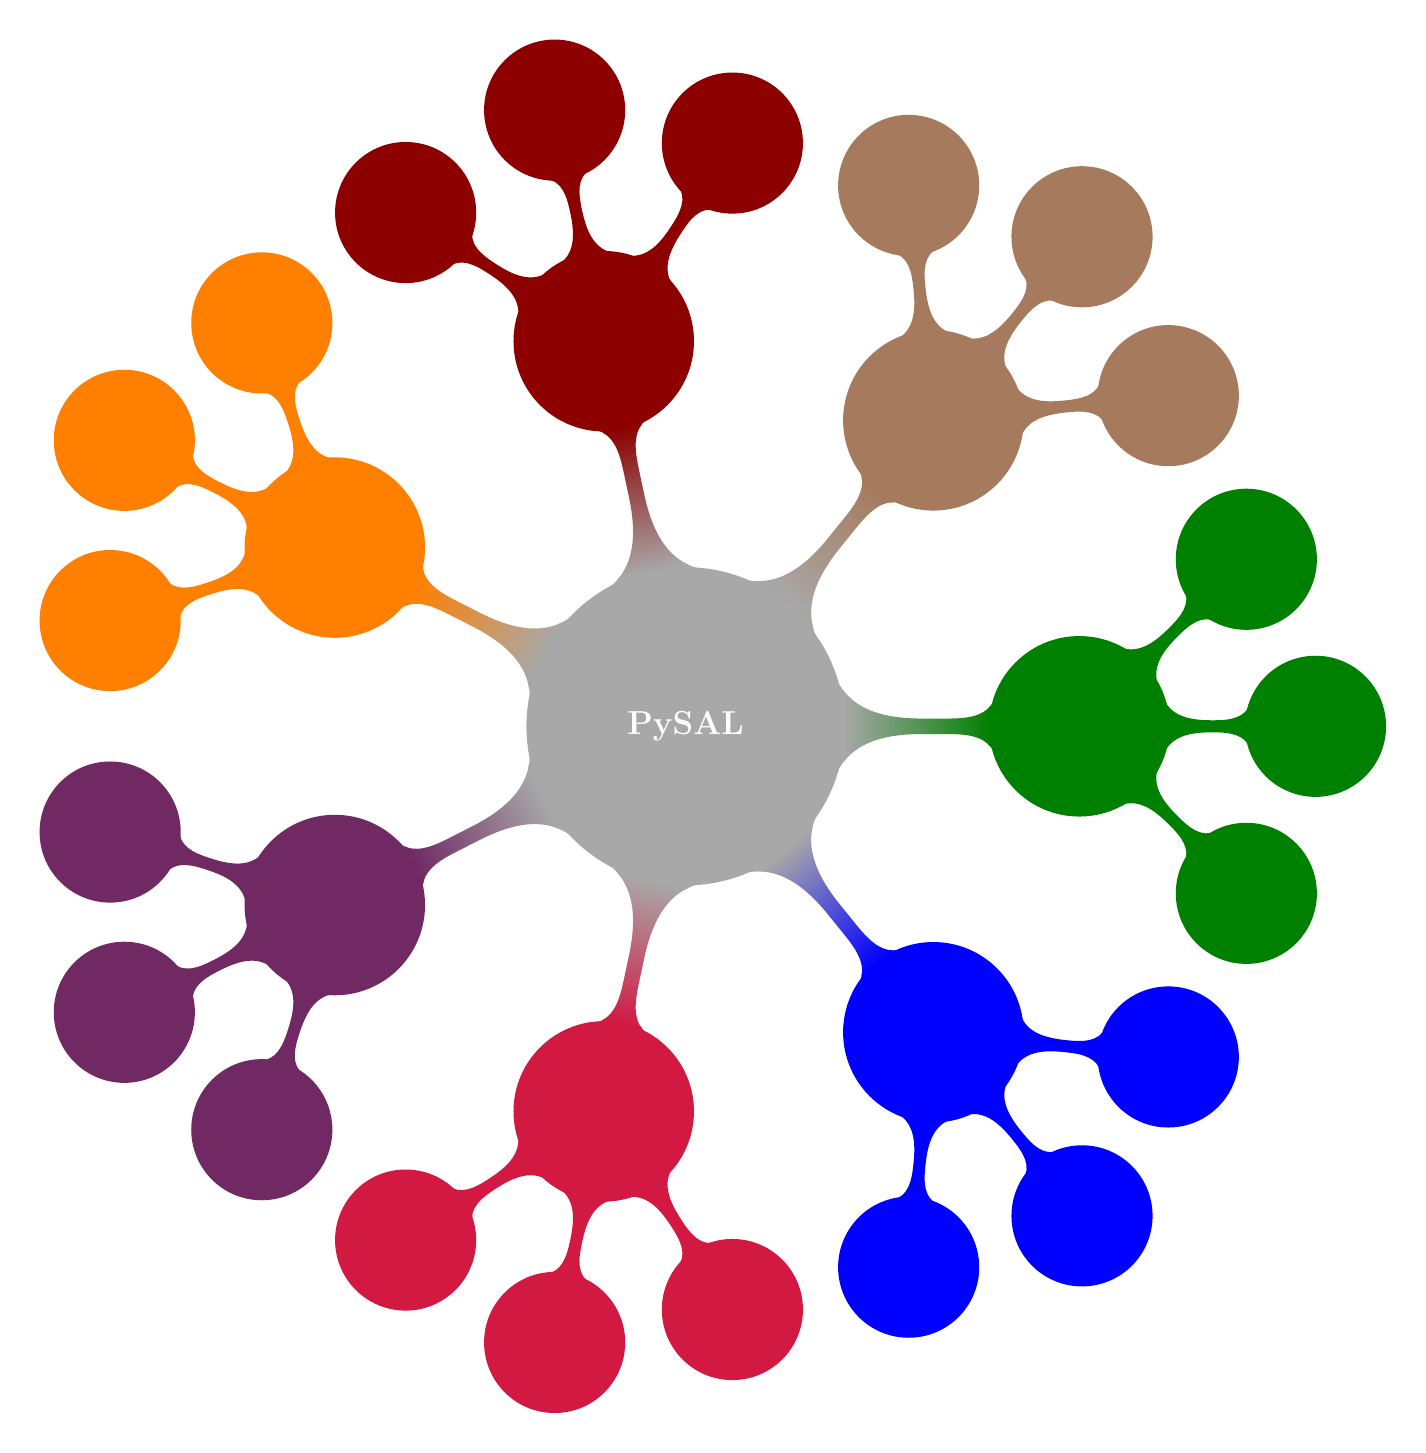
\begin{tikzpicture}[
        background rectangle/.style={fill=white},
        show background rectangle,
        mindmap,
        grow cyclic,
        every node/.style=concept,
        concept color=darkgray,
        text=white,
        level 1/.append style={
            level distance=5cm,
            sibling angle=51,
            font=\Huge
        },
        level 2/.append style={
            level distance=3cm,
            sibling angle=45
        }
    ]
    
        \node[concept color=darkgray]{\large\bfseries{PySAL}}
        child [concept color=byzantium]{ node {}
            child { node { }}
            child { node { }}
            child { node { }}
         }
        child [concept color=alizarin]{ node {}
            child { node { }}
            child { node { }}
            child { node { }}
         }
        child [concept color=blue]{ node {}
            child { node { }}
            child { node { }}
            child { node { }}
         }
        child [concept color=green(html/cssgreen)]{ node {}
            child { node { }}
            child { node { }}
            child { node { }}
         }
        child [concept color=frenchbeige]{ node {}
            child { node { }}
            child { node { }}
            child { node { }}
         }
        child [concept color=darkred]{ node {}
            child { node { }}
            child { node { }}
            child { node { }}
         }
        child [concept color=orange(colorwheel)]{ node {}
            child { node { }}
            child { node { }}
            child { node { }}
         }
                ;
    \end{tikzpicture}
    \end{document}